% !TeX root = ./user_manual.tex
\documentclass[../../report.tex]{subfiles}

\begin{document}

\chapter{User manual: \texttt{recap} package}
\label{chap:user_man_recap}

\emph{Recap} is a tool for providing \emph{REproducible Configurations for Any Project}.
Research should be reproducible.
Especially in deep learning, it is important to keep track of hyperparameters and configurations used in experiments.
This package aims at making that easier.

\section{Installing}
\label{sec:recap_installation}
Before installing this package, ensure that Python version 3.6 or greater is installed on your system.
Furthermore, ensure that the Python package installer \texttt{pip} is installed.

The preferred way of installing this package is to install it directly from \gls{pypi} by running the command:
\begin{minted}{bash}
pip install recap
\end{minted}

However, if you wish to install it from source, you may do so using the \emph{Poetry} tool for managing Python dependencies:
\begin{minted}{bash}
pip install poetry
cd recap
poetry install
poetry shell
\end{minted}
Using Poetry will automatically create a virtual Python environment for this project.
Running \mintinline{bash}|poetry shell| at the end opens a shell in the virtual environment. 
Ensure that you use this shell when running any of the other commands below.

Finally, if you just want to install \texttt{recap} globally without using Poetry, you may instead run:
\begin{minted}{bash}
cd recap
pip install .
\end{minted}

\section{Usage}
Recap provides two top-level concepts that can be imported as follows:
\begin{minted}{python3}
from recap import URI, CfgNode as CN
\end{minted}

The \py{CfgNode} is a subclass of \py{CfgNode} from the \emph{yacs} package.
It provides some additional features for parsing configurations that are inherited between files which is not possible with yacs.

Recap's \py{URI} class provides a mechanism for handling logical paths within your project more conveniently with an interface that is fully compatible with \py{pathlib.Path}.

\subsection{\Acs{yaml} configurations}
Configurations are defined just like in yacs, except that you need to import the \py{CfgNode} class from the recap package instead of yacs.
Consider the following \gls{yaml} configuration that sets default values for all configuration options we will use in our project.
We shall name it \texttt{\_base.yaml} because our experiments will build on these values.
\begin{minted}{yaml}
SYSTEM:
  NUM_GPUS: 4
  NUM_WORKERS: 2
TRAIN:
  LEARNING_RATE: 0.001
  BATCH_SIZE: 32
  SOME_OTHER_HYPERPARAMETER: 10
\end{minted}

The equivalent configuration can be obtained programatically like so:

\begin{minted}{python3}
from recap import CfgNode as CN

cfg = CN()
cfg.SYSTEM = CN()
cfg.SYSTEM.NUM_GPUS = 4
cfg.SYSTEM.NUM_WORKERS = 2
cfg.TRAIN = CN()
cfg.TRAIN.LEARNING_RATE = 1e-3
cfg.TRAIN.BATCH_SIZE = 32
cfg.TRAIN.SOME_OTHER_HYPERPARAMETER = 10
print(cfg)
\end{minted}

\subsubsection{Inheriting configurations}
Recap provides functionality for inheriting configuration options from other configuration files by setting the top-level \mintinline{yaml}{_BASE_} key.
So, we could create a configuration file \path{experiment_1.yaml} for an experiment where we try a different learning rate and batch size:

\begin{minted}{yaml}
_BASE_: _base.yaml

TRAIN:
  LEARNING_RATE: 1e-2
  BATCH_SIZE: 64
\end{minted}

In our code, when we want to load the experiment configuration, we would use the \py{recap.CfgNode.load_yaml_with_base()} function:

\begin{minted}{python3}
from recap import CfgNode as CN

cfg = CN.load_yaml_with_base("experiment_1.yaml")

print(cfg)

# Will output:
"""
SYSTEM:
  NUM_GPUS: 4
  NUM_WORKERS: 2
TRAIN:
  LEARNING_RATE: 0.01
  BATCH_SIZE: 64
  SOME_OTHER_HYPERPARAMETER: 10
"""
\end{minted}
Note that the \mintinline{yaml}{_BASE_} keys can be arbitrarily nested;
however, circular references are prohibited.

\subsection{Logical \acsp{uri} and the path manager}
\label{sec:recap_uris}
Recap includes a path manager for conveniently specifying paths to logical entities.
The path strings are set up like a \gls{uri} where the scheme (i.e.\ \texttt{http} in the path string \texttt{http://google.com}) refers to a logical entity.
Each such entity needs to be set up as a \py{PathTranslator} that can translate the logical \gls{uri} path to a physical path on the file system.

For example, we could set up a path translator for the data scheme to refer to the the path of a dataset on our file system located at \path{/path/to/dataset}. Then the recap URI \path{data://train/abc.txt} would be translated to the local path \path{/path/to/dataset/train/abc.txt}.
The simplest way of setting that up is using the \py{register_translator} function (although more complex setups are possible with the \py{PathTranslator} class, allowing you to download files from the internet, for example):

\begin{minted}{python3}
from recap.path_manager import register_translator
from pathlib import Path

register_translator("data", Path("/path/to/dataset"))
\end{minted}
Then, we can use the \py{recap.URI} class just like any \py{pathlib.Path} object:
\begin{minted}{python3}
from recap import URI

my_uri = URI("data://train/abc.txt")
# Here, str(my_uri) == "/path/to/dataset/train/abc.txt"

with my_uri.open("r") as f:
    print(f.read())
\end{minted}


\subsubsection{Logical \acsp{uri} in inherited configurations}
The \py{recap.URI} interface is fully compatible with nested configurations.
This means that you can use recap \glspl{uri} within the \mintinline{yaml}{_BASE_} field for inheriting configurations.
For example, you could register a path translator for the config scheme and then include \mintinline{yaml}{_BASE_: config://_base.yaml} in your configuration files.

\section{Automated tests}
\label{sec:recap_tests}
To run the automated tests, navigate to the \texttt{recap} folder and then run
\begin{minted}{bash}
python -m pytest
\end{minted}
Note that this will not work if the \texttt{recap} package was installed directly via \texttt{pip} because that will not copy over the \texttt{tests} folder.
Instead, use one of the other two installation options given in \cref{sec:recap_installation}
Ensure that \texttt{poetry shell} is run before executing this command if the package was installed via Poetry.
A screenshot of the output is provided in \cref{lst:tests_recap}.

\section{Documentation}
\label{sec:recap_documentation}
More detailed documentation than this user manual is available at \url{https://recap.readthedocs.io}.
The package documentation includes detailed explanations of each of the submodules, methods, and classes.
The same documentation is provided in \gls{html} format alongside this submission at \path{docs/recap/index.html}.

\chapter{User manual: \texttt{chesscog}}
\label{chap:user_man_chesscog}

\emph{Chesscog} combines traditional computer vision techniques with deep learning to identify chess positions from photos.
This repository contains all the code required to execute the chess recognition pipeline end-to-end as well as to train and fine-tune the \glspl{cnn} for unseen chess sets.
Furthermore, the evaluation scripts for the experiments conducted for this report are available in this package.

\section{Installing}
\label{sec:chesscog_installing}
Before installing this package, ensure that Python version 3.7 or greater is installed on your system.
Furthermore, ensure that the Python package installer \texttt{pip} is installed.
Then, navigate to the \texttt{chesscog} folder in the submission, or run \mintinline{bash}{git clone https://github.com/georgw777/chesscog.git}.

The easiest way to install the \texttt{chesscog} package and its dependencies is to run:
\begin{minted}{bash}
pip install .
\end{minted}

However, if you wish to install it using the \emph{Poetry} tool for managing Python dependencies, first ensure that Poetry is installed by running \mintinline{bash}{pip install poetry} and then run:
\begin{minted}{bash}
cd chesscog
poetry install
poetry shell
\end{minted}
Using Poetry will automatically create a virtual Python environment for this project.
Running \mintinline{bash}|poetry shell| at the end opens a shell in the virtual environment. 
Ensure that you use this shell when running any of the other commands below.

\section{Usage}

As explained in \cref{sec:chesscog_implementation}, many Python files simultaneously act as scripts.
The following subsections provide instructions for running these scripts in order to carry out the main tasks of the chess recognition system.
The scripts themselves are explained in more detail in the documentation (see \cref{sec:chesscog_documentation}), but are also self-documenting when supplied with the \texttt{--help} command line option.

\subsection{Dataset}
\label{sec:user_man_chesscog_dataset}

The recommended method of obtaining the rendered dataset is by following the instructions in \cref{sec:user_man_chesscog_download_dataset} to download it.
However, for the sake of completeness, the following subsection details how the script used to generate the dataset was run.

\subsubsection{Data synthesis}
To synthesise the 3D dataset, first install Blender. 
Then, the \texttt{chess} library must be installed in Blender's own Python interpreter.
On a Mac, this can be achieved by running:
\begin{minted}{bash}
cd /Applications/Blender.app/Contents/Resources/2.90/python/bin
./python3.7m -m ensurepip
./python3.7m -m pip install --upgrade pip
./python3.7m -m pip install chess
\end{minted}

Finally, from back in the \texttt{chesscog} directory, the data can be synthesised using the following command:
\begin{minted}{bash}
blender chess_model.blend --background --python scripts/synthesize_data.py
\end{minted}
Note that this requires the \texttt{chess\_model.blend} file, i.e.\ the 3D chess model as a Blender file.
However, this model is not supplied with the project submission due to its large file size.

\subsubsection{Downloading and splitting the dataset}
\label{sec:user_man_chesscog_download_dataset}
To download the dataset and then perform the train/val/test split, run the two following commands:
\begin{minted}{bash}
python -m chesscog.data_synthesis.download_dataset
python -m chesscog.data_synthesis.split_dataset
\end{minted}
The dataset will be downloaded to the \path{data://render} folder which by default maps to \path{~/chess_data} (the mapping is achieved using \texttt{recap}'s \acs{uri} interface detailed in \cref{sec:recap_uris}).
This directory contains three subfolders, \texttt{train}, \texttt{val}, and \texttt{test}.

\subsubsection{Format of the dataset}
In each of the three subfolders, the images are supplied in PNG format.
For every image file, there is a \gls{json} file with the same name (but \texttt{*.json} extension) that contains the associated labels.
The contents of that \gls{json} file is shown in \cref{lst:json_labels} for the running example in \cref{chap:data_synthesis}.
\begin{listing}
    \inputminted{json}{\subfix{../../data/3828.json}}
    \caption[\acs{json} format of the annotations generated for the running example image from \cref{chap:data_synthesis}.]{\acs{json} format of the annotations generated for the running example image from \cref{chap:data_synthesis} (see \cref{fig:data_synthesis_visualisation}).}
    \label{fig:json_labels}
\end{listing}
Training of the chess recognition system relies only on the \texttt{fen}, \texttt{white\_turn}, and \texttt{corners} fields which respectively provide the \gls{fen} description of the chess position on the board, the colour of the current player (indicating from which player's perspective the photo was taken), and the pixel coordinates of the chessboard's four corner points.
The origin of the coordinate system is the top left of the image.

Nonetheless, the \gls{json} file also contains information about the positions and rotations of the lights and camera in the 3D world coordinate system as explained in \cref{sec:3d_renders}.
Furthermore, the bounding boxes for each of the pieces on the board are given in the \texttt{pieces} field in the \gls{json} file.
The coordinates are supplied in the order $x_1,y_1,x_2,y_2$.
This information is useful for potential further research exploring the use of object detection models for chess recognition.

\subsection{Board localisation}
Code related to board localisation is in the \py{chesscog.corner_detection} module.
More specifically, the \py{chesscog.corner_detection.detect_corners} submodule contains the \py{find_corners()} method that takes as input an image (as a \py{numpy} array) and outputs the detected corner points.
This submodule simultaneously acts as a script that can be run as follows:
\begin{minted}{bash}
python -m chesscog.corner_detection.detect_corners img.png
\end{minted}
Here, \texttt{img.png} is to be replaced with the path to the input image.
\Cref{fig:example_detect_corners} shows the output of that script when supplied with the path \path{data://render/train/3828.png} which is the running example from \cref{chap:data_synthesis}.
\begin{figure}
    \centering
    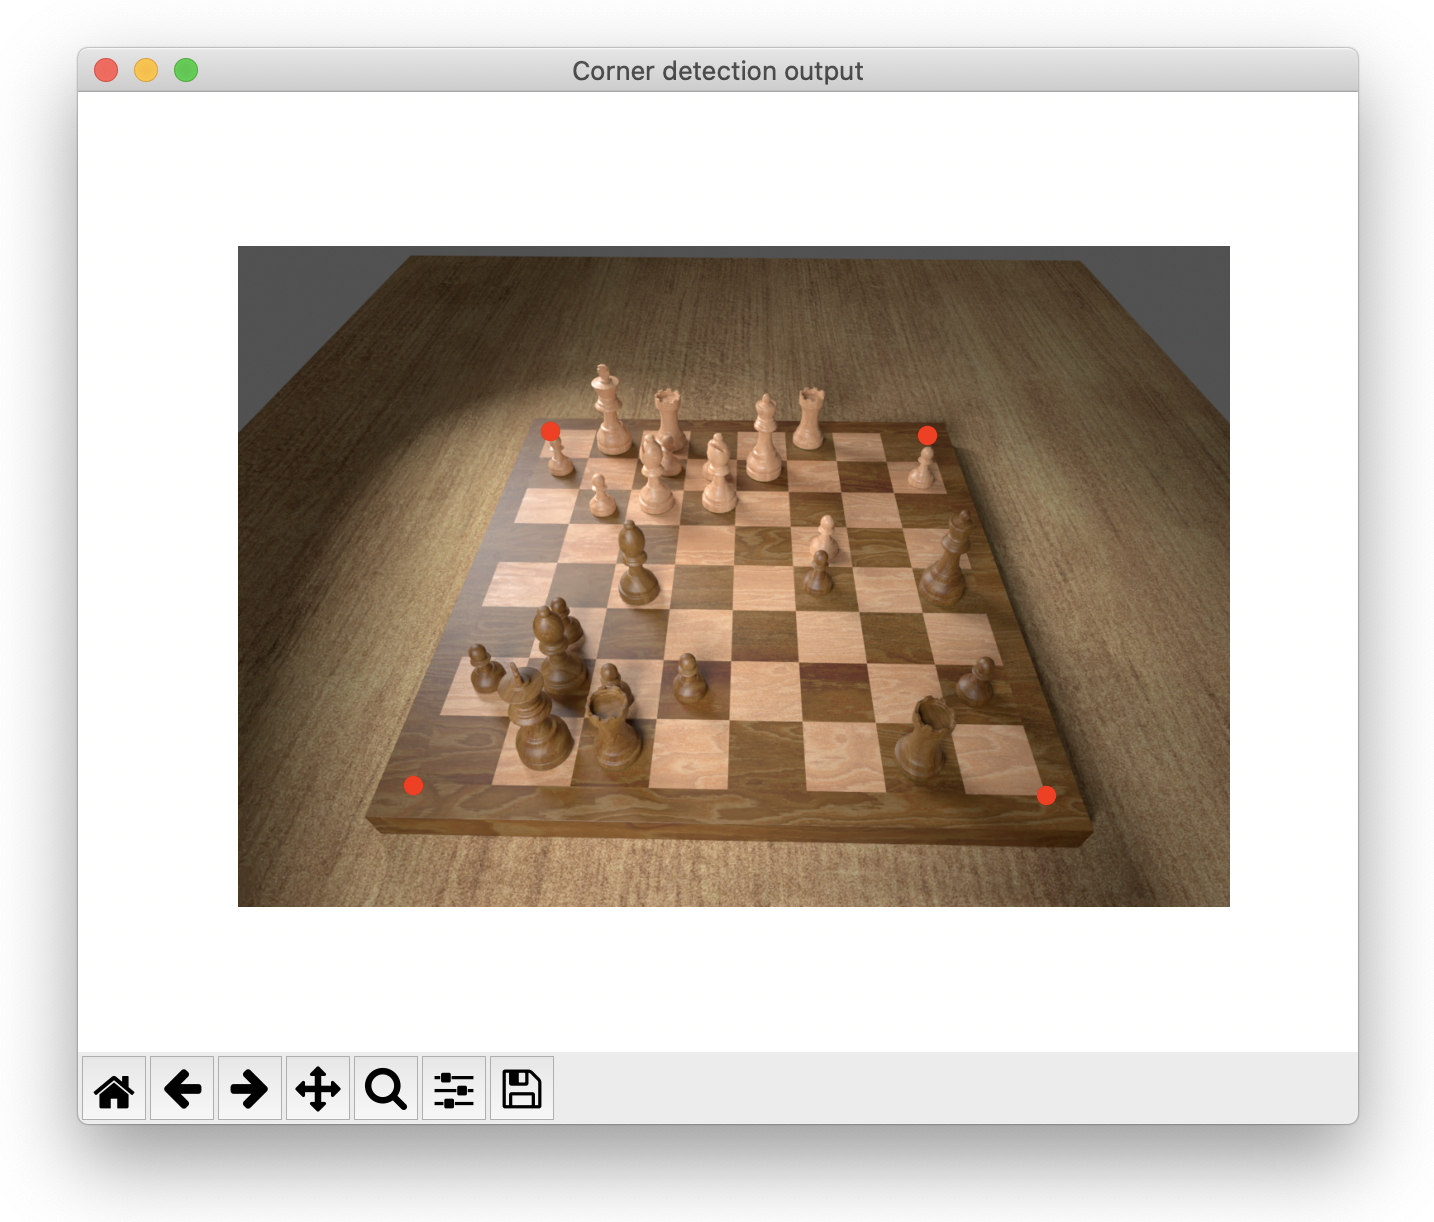
\includegraphics[width=.8\textwidth]{3828_corner_detection_screenshot}
    \caption{Screenshot of the corner detection script's output.}
    \label{fig:example_detect_corners}
\end{figure}

\subsection{Occupancy and piece classification}
Code for training and evaluating the occupancy and piece classifiers is located in the \py{chesscog.occupancy_classifier} and \py{chesscog.piece_classifier} modules respectively.
\subsubsection{Downloading the trained models}
To download the trained models, simply run:
\begin{minted}{bash}
python -m chesscog.occupancy_classifier.download_model
python -m chesscog.piece_classifier.download_model
\end{minted}
The models are downloaded to the \path{models://occupancy_classifier} and \path{models://piece_classifier} folders.
To find out where that is on the local file system, run the following little Python script:
\begin{minted}{python3}
import recap
import chesscog # must be imported to properly configure recap
print(recap.URI("models://"))
\end{minted}
\subsubsection{Training the models}
To train the models yourself instead of using the already trained models (see previous section), the relevant datasets of the cropped squares must first be created by running:
\begin{minted}{bash}
python -m chesscog.occupancy_classifier.create_dataset
python -m chesscog.piece_classifier.create_dataset
\end{minted}
Then, the models can be trained by running:
\begin{minted}{bash}
python -m chesscog.occupancy_classifier.train
python -m chesscog.piece_classifier.train
\end{minted}
This will train all models specified using \gls{yaml} configuration files in the \path{config://occupancy_classifier} and \path{config://piece_classifier} folders.
It is recommended that you use a machine with a CUDA-compatible \gls{gpu} for training.
To inspect the progress, run in a separate shell:
\begin{minted}{bash}
tensorboard --logdir ./runs
\end{minted}
The TensorBoard tool plots the key metrics live during training.
It should already be installed if you followed the instructions in \cref{sec:chesscog_installing}.
Finally, you should copy the folder of your selected piece and occupancy classifiers from \path{./runs} into \path{models://} so that these models will be used for inference and evaluation.

\subsection{Performing an inference}
The \py{chesscog.recognition} module is responsible for running the chess recognition pipeline end to end.
Further, the \py{chesscog.recognition.recognition} submodule provides the \py{ChessRecognizer} class that upon initialisation will load the \glspl{cnn} into memory and exposes the \py{predict()} method that when supplied with an input image will return the predicted \gls{fen} description.
This submodule also acts as a script that can be executed as follows:
\begin{minted}{bash}
python -m chesscog.recognition.recognition img.png --white
\end{minted}
Again, \texttt{img.png} should be replaced by the path to the desired input image (which may be a \texttt{recap} \gls{uri}).
The \texttt{--white} flag specifies the current player's perspective and can be replaced with \texttt{--black} for the other player.
\Cref{lst:chesscog_recognition_output} shows the output of that script.
\begin{listing}
    \verbatiminput{data/recognition_output.txt}
    \caption[Output of the chess recognition script.]{Output of the chess recognition script. Additional line breaks that were added to fit on the page are indicated with a backslash.}
    \label{lst:chesscog_recognition_output}
\end{listing}
It provides the user with a text-based representation of the predicted chess position and a link to the chess engine analysis tool on the popular chess website \emph{Lichess} with that position set up.

\subsection{Performance evaluation}
For evaluating the performance of the entire chess recognition pipeline on the test set, run:
\begin{minted}{text}
python -m chesscog.recognition.evaluate --save-fens --dataset test
\end{minted}
This creates a \gls{csv} file at \path{results://recognition/test.csv} that contains the prediction result (as well as other information like the number of mistakes) for each sample in the test set.
To obtain an overview of useful metrics (those shown in \cref{tbl:chess_recognition_trainvaltest_results}), run:
\begin{minted}{text}
python -m chesscog.report.prepare_recognition_results \
  --results results://recognition --dataset test
\end{minted}

The \py{chesscog.corner_detection}, \py{chesscog.occupancy_classifier}, and \py{chesscog.piece_classifier} each contain an \texttt{evaluate} module that acts in a similar manner to that of the whole system described above.
These modules facilitate the separate performance evaluation of the individual components of the pipeline.
For more information, run these models with the \texttt{--help} flag.

\subsection{Adapting to an unseen chess set}

\section{Automated tests}
\label{sec:chesscog_tests}

\section{Documentation}
\label{sec:chesscog_documentation}

\chapter{User manual: web app}
\label{chap:user_man_chesscogapp}

\section{Installing}
\section{Usage}
\section{Automated tests}
\label{sec:chesscogapp_tests}
\section{Documentation}
FaQ page


\end{document}